\documentclass[12pt,compress,aspectratio=169]{beamer}
\usetheme{metropolis}
\setbeamersize{text margin left=.5cm,text margin right=.5cm}
\usepackage[lf]{carlito}
\usepackage{siunitx}
\usepackage{tikz}
\usepackage{mathpazo}
\usepackage{bm}

\usetikzlibrary{decorations.pathmorphing,patterns}

\setlength{\parskip}{0pt}
\setlength{\itemsep}{0pt}
\renewcommand{\baselinestretch}{1}

\sisetup{
  inter-unit-product=\cdot,
  per-mode=symbol
}
\tikzset{
  >=latex,
}

\title{Topic 7: Simple Harmonic Motion}
\subtitle{Advanced Placement Physics 1}
\author[TML]{Dr.\ Timothy Leung}
\institute{Olympiads School}
\date{\today}

\newcommand{\pic}[2]{\includegraphics[width=#1\textwidth]{#2}}
\newcommand{\eq}[2]{\vspace{#1}{\Large\begin{displaymath}#2\end{displaymath}}}

\begin{document}

\begin{frame}
  \maketitle
\end{frame}


\section{Review: Hooke's Law}

\begin{frame}{Review: Hooke's Law}
  \textbf{Hooke's law} relates the force $\bm{F}_s$ (\textbf{spring force})
  exerted by a compressed or stretched spring onto another object to the
  stiffness of the spring $k$ (\textbf{spring constant}, \textbf{Hooke's
    constant} or \textbf{force constant}) and spring displacement $\bm{x}$:

  \eq{-.1in}{
    \boxed{\bm{F}_s=-k\bm{x}}
  }

  \begin{itemize}
  \item\vspace{-.1in}The unit for $k$ is \textbf{newton per meter}
    (\si{\newton\per\metre})
  \item $\bm{F}_s$ is a \textbf{restoring force}: its direction is always
    opposite to the displacement to always move it back towards $\bm{x}=0$.
  \item The magnitude of $\bm{F}_s$ is non constant: the acceleration of
    objects connected to it changes with time
  \end{itemize}
\end{frame}



\begin{frame}{Elastic Potential Energy}
  Applying Hooke's law to the  definition of work ($W=F\Delta x$), and after a
  bit of simple calculus, we find that a compressed/stretched spring stores
  \textbf{elastic potential energy}:
  
  \eq{-.1in}{
    \boxed{U_e=\frac12kx^2}
  }

  The spring force is a conservative force.
\end{frame}



\section{Spring-Mass Systems}

\begin{frame}{Mass on a Spring}
  Consider the forces acting on a mass connected horizontally to a spring

  \begin{center}
    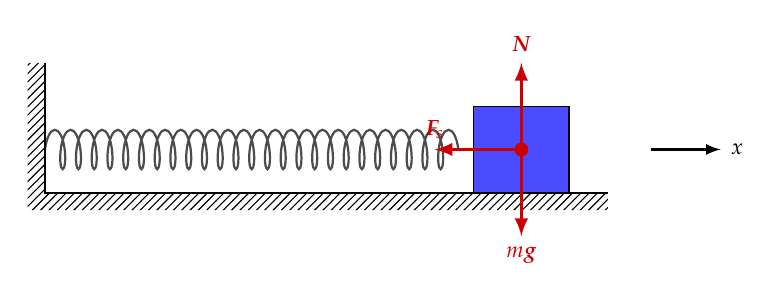
\begin{tikzpicture}[scale=1.1]
      \draw[fill=blue!70] (4.95,.5) rectangle (6.05,1.5); %{$m$};
      \draw[thick,draw=black!70,
        decoration={aspect=.3,segment length=2mm, amplitude=2.5mm, coil},
        decorate] (0,1)--(4.95,1);
      \fill[pattern=north east lines] (6.5,.5)--(6.5,.3)--(-0.2,.3)
      --(-.2,2)--(0,2)--(0,.5)--cycle;
      \draw[thick] (6.5,.5)--(0,.5)--(0,2);
      \draw[->,thick](7,1)--(7.8,1) node[right]{\footnotesize $x$};
      
      \fill[red!80!black] (5.5,1) circle(.08);
      \begin{scope}[very thick,->,red!80!black]
        \draw (5.5,1)--(5.5,0) node[below]{\footnotesize $m\bm{g}$};
        \draw (5.5,1)--(5.5,2) node[above]{\footnotesize $\bm{N}$};
        \draw (5.5,1)--(4.5,1) node[above]{\footnotesize $\bm{F}_s$};
      \end{scope}
    \end{tikzpicture}
  \end{center}

  \vspace{-.1in}$m\bm{g}$ and $\bm{N}$ cancel out, so net force is due only to
  spring force $\bm{F}_s=-k\bm{x}$ along the $x$-axis. This is true both when
  the spring is in compression or extension. (The spring is in extension in the
  diagram.)
\end{frame}



\begin{frame}{Horizontal Spring-Mass System}
  Applying second law of motion in the $x$-direction results in an equation
  containing both displacement and acceleration:

  \eq{-.2in}{
    \sum F=F_s=ma\quad\rightarrow\quad-\frac{k}mx=a
  }

  We know that:
  \begin{itemize}
  \item Velocity is how quickly position changes in time, and
  \item Acceleration is how quickly velocity changes in time
  \end{itemize}
  So the left \& right hand side of this equation are actually related. In
  calculus, we call this a
  \emph{second-order ordinary differential equation with constant coefficients}.
\end{frame}



\begin{frame}{Horizontal Spring-Mass System}
  Solving this equation is something  every calculus student have to learn. The
  general form of the solution is the cosine (or sine) function:

  \eq{-.25in}{
    x(t)=A\cos(\omega t-\phi)
  }

  \vspace{-.1in}where $\omega$ is the \textbf{angular frequency}, $A$ is the
  amplitude of the oscillation and $\phi$ is a \textbf{phase shift} (or
  \textbf{phase constant}) that depends on the initial condition
  
  \vspace{.15in}$\cos$ is preferred over $\sin$ because $\cos(0)=1$,
  consistent with the fact that oscillations usually begin at maximum amplitude
  $A$ at $t=0$ and we can set $\phi=0$. Mathematically, the two functions only
  differ in $\phi=\pi/2$
\end{frame}


\begin{frame}{Horizontal Spring-Mass System}
  Starting with the general form and applying some differential calculus, we
  obtain the velocity and acceleration of the mass as functions of time:
 
  \vspace{-.35in}{\Large
    \begin{align*}
      x(t)&=A\cos(\omega t-\phi)\\
      v(t)&=-A\omega\sin(\omega t-\phi)\\
      a(t)&=-A\omega^2\cos(\omega t-\phi)=-\omega^2x
    \end{align*}
  }

  Acceleration can be expressed as function of time or a function of position.
\end{frame}



\begin{frame}{Angular Frequency}
  Comparing these two expressions

  \eq{-.2in}{
    a(t)=-\omega^2x(t)\quad\quad -kx(t)=ma(t)
  }
  
  It is obvious that the angular frequency $\omega$ must be related to the
  spring constant and mass. The angular frequency for the (undamped) simple
  harmonic oscillator is called the \textbf{natural frequency}:

  \eq{-.15in}{
    \boxed{\omega=\sqrt{\frac{k}m}}
  }
\end{frame}



\begin{frame}{Frequency and Period of a Spring-Mass System}
  The period $T$ and frequency $f$ of the simple harmonic motion are given by:

  \eq{-.1in}{
    \boxed{f=\frac{\omega}{2\pi}=\frac1{2\pi}\sqrt{\frac{k}m}}
    \quad\quad
    \boxed{T=\frac1f=2\pi\sqrt{\frac{m}k}}
  }
  
  Angular frequency $\omega$, frequency $f$ and period $T$ are independent
  of amplitude $A$
\end{frame}



\begin{frame}{Vertical Spring-Mass System}
  \vspace{.2in}
  \begin{columns}
    \column{.2\textwidth}
    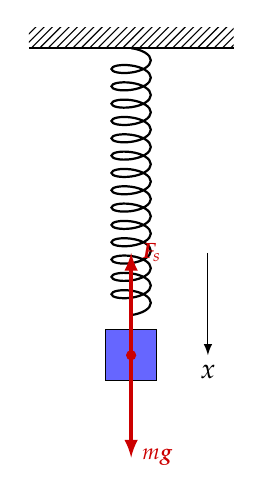
\begin{tikzpicture}[scale=1.3]
      \draw[fill=blue!60] (.75,1.75) rectangle (1.25,2.25);
      \draw[thick,
        decoration={aspect=.4,segment length=2.2mm, amplitude=2.5mm, coil},
        decorate] (1,5)--(1,2.25); 
      \fill [pattern=north east lines] (0,5) rectangle (2,5.2);
      \draw[thick] (0,5)--(2,5);
      \draw[->](1.75,3)--(1.75,2) node[below]{$x$};
      \begin{scope}[very thick,->,red!80!black]
        \draw(1,2)--(1,1)node[right]{\footnotesize $m\bm{g}$};
        \draw(1,2)--(1,3)node[right]{\footnotesize $\bm{F}_s$};
      \end{scope}
      \fill[red!80!black](1,2) circle(.05);
    \end{tikzpicture}

    \column{.8\textwidth}
    For a vertical spring-mass system, we must consider the weight $m\bm{g}$
    of the mass as well, but since weight is constant, the only change is the
    addition of a constant $B$ in the expression of $x(t)$:
    
    \vspace{-.4in}{\Large
      \begin{align*}
        x(t)&=A\cos(\omega t-\phi) +B\\
        v(t)&=-A\omega\sin(\omega t-\phi)\\
        a(t)&=-A\omega^2\cos(\omega t-\phi)
      \end{align*}
    }
    There is no change in the expressions for $v(t)$ and $a(t)$.
  \end{columns}
\end{frame}



\begin{frame}{Vertical Spring-Mass System}
  \vspace{.2in}
  \begin{columns}
    \column{.2\textwidth}
    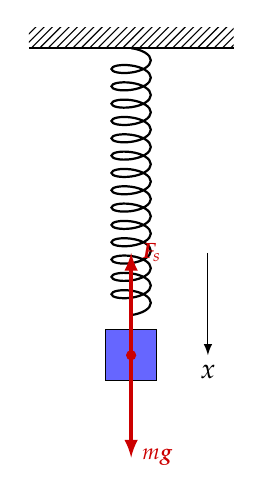
\begin{tikzpicture}[scale=1.3]
      \draw[fill=blue!60] (.75,1.75) rectangle (1.25,2.25);
      \draw[thick,
        decoration={aspect=.4,segment length=2.2mm, amplitude=2.5mm, coil},
        decorate] (1,5)--(1,2.25); 
      \fill [pattern=north east lines] (0,5) rectangle (2,5.2);
      \draw[thick] (0,5)--(2,5);
      \draw[->](1.75,3)--(1.75,2) node[below]{$x$};
      \begin{scope}[very thick,->,red!80!black]
        \draw(1,2)--(1,1) node[right]{\footnotesize $m\bm{g}$};
        \draw(1,2)--(1,3) node[right]{\footnotesize $\bm{F}_s$};
      \end{scope}
      \fill[red!80!black](1,2) circle(.05);
    \end{tikzpicture}

    \column{.8\textwidth}
    The constant $B$ is the amount that the equilibrium position is stretched
    downwards, and is the stretching of the spring due to its weight:
    
    \eq{-.23in}{
      B=\frac{mg}k
    }

    Angular frequency (natural frequency) is the same as the horizontal case:

    \eq{-.23in}{
      \omega=\sqrt{\frac{k}m}
    }
  \end{columns}
\end{frame}



\begin{frame}{Conservation of Energy in a Spring-Mass System}

  In spring-mass systems, assuming no frictional losses, then the only
  forces doing work are the spring force (horizontal and vertical) and gravity
  (vertical). Both forces are \emph{conservative}, therefore total mechanical
  energy is conserved:

  \eq{-.2in}{
    K + U_e + U_g = K' + U_e' + U_g'
  }
  
  For the horizontal spring-mass system, the total energy of the simple harmonic
  oscillator is:
    
  \eq{-.2in}{
    \boxed{E_T=\frac12kA^2}
  }
\end{frame}


\begin{frame}{Simple Example}
  \textbf{Example 2:} A mass suspended from a spring is oscillating up and
  down. Consider the following two statements:
  \begin{enumerate}
  \item At some point during the oscillation, the mass has zero velocity but it
    is accelerating
  \item At some point during the oscillation, the mass has zero velocity and
    zero acceleration.
  \end{enumerate}

  \begin{enumerate}[(a)]
  \item Both occur at some time during the oscillation
  \item Neither occurs during the oscillation
  \item Only (1) occurs
  \item Only (2) occurs
  \end{enumerate}
\end{frame}



\begin{frame}{Another Example}
  \textbf{Example 3:} An object of mass \SI5{\kilo\gram} hangs from a spring
  and oscillates with a period of \SI{.5}\second. By how much will the
  equilibrium length of the spring be shortened when the object is removed.
  \begin{enumerate}[(a)]
  \item\SI{0.75}{\centi\metre}
  \item\SI{1.50}{\centi\metre}
  \item\SI{3.13}{\centi\metre}
  \item\SI{6.21}{\centi\metre}
  \end{enumerate}
\end{frame}



\section{Simple Pendulum}

\begin{frame}{What About a Simple Pendulum?}
  \begin{columns}
    \column{.75\textwidth}
    \begin{itemize}
    \item Pendulums also exhibit oscillatory motion
    \item A \textbf{simple pendulum} is where the mass is concentrated at the
      end point
    \item There are two forces acting on the mass: weight $mg$ and tension $T$
    \item When the mass is deflected by $\phi$, the component of gravity in
      the tangential direction is $F_t=-mg\sin\phi$
    \item No need to worry about the radial direction because it does not
      have to do with the restoring force
    \end{itemize}
    %(I am running out of Greek letters for angles!)
    
    \column{.25\textwidth}
    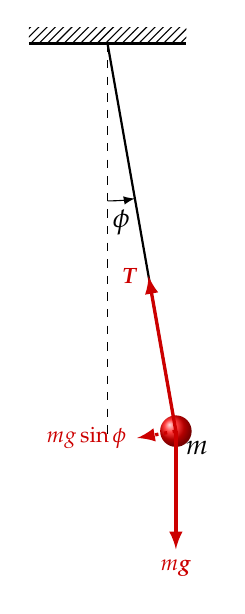
\begin{tikzpicture}
      \fill[pattern=north east lines] (-1,0) rectangle (1,0.2);
      \draw[thick](-1,0)--(1,0);
      \begin{scope}[rotate=10]
        \draw[thick](0,0)--(0,-5);
        \tikzstyle{balloon}=[ball color=red];
        \shade[balloon] (0,-5) circle (.2) node[below right]{$m$};
        \begin{scope}[very thick,->,red!80!black]
          \draw[dotted](0,-5)--(-0.5,-5)node[left]{\footnotesize $mg\sin\phi$};
          \draw (0,-5)--(0,-3) node[left]{\footnotesize $\bm{T}$};
          \draw[rotate around={-10:(0,-5)}](0,-5)--(0,-6.5)
          node[below]{\footnotesize $m\bm{g}$};
        \end{scope}
      \end{scope}
      \draw[dashed,thin](0,0)--(0,-5);
      \draw[->](0,-2) arc(270:280:2) node[midway,below]{$\phi$};
    \end{tikzpicture}
  \end{columns}
\end{frame}



\begin{frame}{The Simple Pendulum}
  \begin{columns}
    \column{.75\textwidth}
    Substitute $F_t$ into the second law of motion, and cancelling mass term,
    we get:

    \eq{-.2in}{
      F_t=ma_t\;\;\rightarrow\;\; -g\sin\phi=\ell\alpha
    }

    \vspace{-.1in}where the acceleration $\alpha$ is the angular acceleration
    $\alpha$, and tangential acceleration is $a_t=\ell\alpha$. Solving this ODE
    is difficult because of the $\sin\phi$ term. However, using the series
    expansion of the sine function

    \eq{-.2in}{
      \sin\phi=\phi-\frac{\phi^3}{3!}+\frac{\phi^5}{5!}-
      \frac{\phi^7}{7!}+\cdots
    }
    
    shows that for ``small angles'' (usually <\ang{10}), $\sin\phi\approx\phi$
    
    \column{.25\textwidth}
    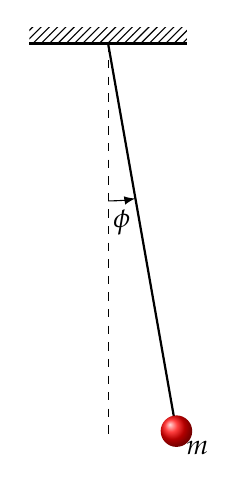
\begin{tikzpicture}
      \fill[pattern=north east lines] (-1,0) rectangle (1,0.2);
      \draw[very thick](-1,0)--(1,0);
      \begin{scope}[rotate=10]
        \draw[thick](0,0)--(0,-5);
        \tikzstyle{balloon}=[ball color=red];    
        \shade[balloon] (0,-5) circle (0.2) node[below right]{$m$};
      \end{scope}
      \draw[dashed,thin](0,0)--(0,-5);
      \draw[->](0,-2) arc(270:280:2) node[midway,below]{$\phi$};
    \end{tikzpicture}
  \end{columns}
\end{frame}



\begin{frame}{The Simple Pendulum}
  \begin{columns}
    \column{.75\textwidth}
    For small angles of $\phi$, the equation that needs to be solved is
    essentially the same as the spring-mass system:

    \eq{-.2in}{
      -g\phi=\ell\alpha
    }

    \vspace{-.1in}Instead of position $x$ and acceleration $a$, we have
    \emph{angular} position $\phi$ and \emph{angular} acceleration $\alpha$ of
    the pendulum. This expression is similar to the spring-mass case.
    
    \column{.25\textwidth}
    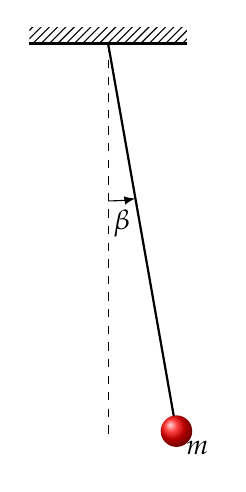
\begin{tikzpicture}
      \fill[pattern=north east lines] (-1,0) rectangle (1,0.2);
      \draw[very thick](-1,0)--(1,0);
      \begin{scope}[rotate=10]
        \draw[thick](0,0)--(0,-5);
        \tikzstyle{balloon}=[ball color=red];    
        \shade[balloon] (0,-5) circle (0.2) node[below right]{$m$};
      \end{scope}
      \draw[dashed,thin](0,0)--(0,-5);
      \draw[->](0,-2) arc(270:280:2) node[midway,below]{$\beta$};
    \end{tikzpicture}
  \end{columns}
\end{frame}



\begin{frame}{Solution for Deflection}
  The solution for $\phi(t)$ is similar to the spring-mass system:

  \eq{-.2in}{
    \boxed{\phi(t)=\Phi\cos(\omega t-\beta)}
  }
    
  where amplitude $\Phi$ is the maximum deflection of the pendulum (less than
  \ang{10}), and angular frequency of the oscillation $\omega$ is given by:
  
  \eq{-.15in}{
    \boxed{\omega=\sqrt{\frac{g}L}}
  }
\end{frame}



\begin{frame}{A Pendulum Example}
  \textbf{Example:} A bucket full of water is attached to a rope and allowed
  to swing back and forth as a pendulum from a fixed support. The bucket has a
  hole in its bottom that allows water to leak out. How does the period of
  motion change with the loss of water?
  \begin{enumerate}[(a)]
  \item The period does not change.
  \item The period continuously decreases.
  \item The period continuously increases.
  \item The period increases to some maximum and then decreases again.
  \end{enumerate}
\end{frame}


\begin{frame}{Think About $g$}
  \textbf{Example:} A little girl is playing with a toy pendulum while riding
  in an elevator. Being an astute and educated young lass, she notes that the 
  period of the pendulum is \SI{.5}\second. Suddenly the cables
  supporting the elevator break and all  of the brakes and safety features fail
  simultaneously. The elevator plunges into free fall. The young girl is
  astonished to discover that the pendulum has:
  \begin{enumerate}[(a)]
  \item continued oscillating with a period of \SI{.5}\second.
  \item stopped oscillating entirely.
  \item decreased its rate of oscillation to have a longer period.
  \item increased its rate of oscillation to have a lesser period.
  \end{enumerate}
\end{frame}



\section{Damped Oscillations}

\begin{frame}{It's Never Perfect}
  In reality, there are friction, or drag, or other forces present in any
  spring-mass system that takes away energy, represented by a shock absorber:
  \begin{center}
    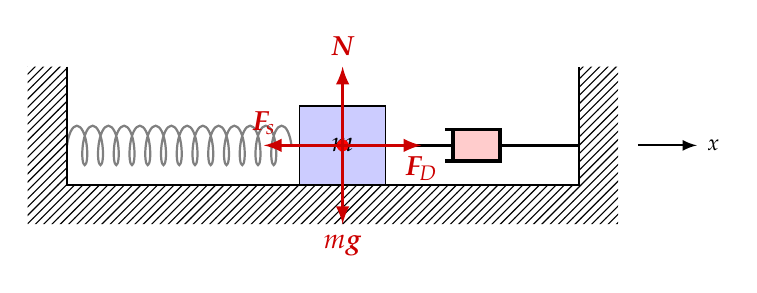
\begin{tikzpicture}
      \draw[fill=blue!20!white] (2.95,.5) rectangle(4.05,1.5)
      node[midway]{$m$};
      \draw[thick,draw=black!50,
        decoration={aspect=0.3,segment length=2mm, amplitude=2.5mm, coil},
        decorate] (0,1)--(2.95,1);
      \fill[pattern=north east lines](-.5,2)--(-.5,0)--(7,0)--(7,2)--(6.5,2)
      --(6.5,.5)--(0,.5)--(0,2)--cycle;
      \draw[thick] (0,2)--(0,.5)--(6.5,.5)--(6.5,2);
      \draw[->,thick](7.25,1)--(8,1) node[right]{\footnotesize $x$};

      %shock absorber
      \draw[fill=red!20!white] (4.9,.8) rectangle(5.5,1.2);
      \begin{scope}[very thick]
        \draw(4.05,1)--(4.9,1);
        \draw(4.9,.8)--(4.9,1.2);
        \draw(4.8,1.2)--(5.5,1.2)--(5.5,.8)--(4.8,.8);
        \draw(5.5,1)--(6.5,1);
      \end{scope}
      
      \uncover<2->{
        \fill[red] (3.5,1)circle(.075);
        \begin{scope}[very thick,->,red!80!black]
          \draw(3.5,1)--(3.5,0) node[below]{$m\bm{g}$};
          \draw(3.5,1)--(3.5,2) node[above]{$\bm{N}$};
          \draw(3.5,1)--(2.5,1) node[above]{$\bm{F}_s$};
          \draw(3.5,1)--(4.5,1) node[below]{$\bm{F}_D$};
        \end{scope}
      }
    \end{tikzpicture}
  \end{center}
  \uncover<2->{
    The damping force is typically proportional to velocity, in the opposite
    direction:

    \eq{-.3in}{
      \bm{F}_D=-b\bm{v}
    }

    \vspace{-.1in}Second law of motion:

    \eq{-.4in}{
      -kx-bv=ma
    }
  }
\end{frame}



\begin{frame}{Damped Oscillator}
  The solution this equation is a standard (albeit more difficult) calculus
  problem. The motion of the mass has both an exponential decay and a
  sinusoidal term:

  \eq{-.2in}{
   x(t)=A_0e^{-\frac{b}{2m}t}\cos(\omega't+\phi)
  }

  \vspace{-.1in}where $A_0$ is the initial amplitude, and angular frequency
  $\omega'$ is now shifted from the natural frequency:

  \eq{-.15in}{
    \omega'=\sqrt{\omega_0^2-\left(\frac{b}{2m}\right)^2}
    \quad{\text{\normalsize where}}\quad
    \omega_0=\sqrt{\frac{k}m}
  }
  
  Angular frequency $\omega'$ of the damped oscillator differs
  from the undamped case $\omega_0$ depending on the damping factor $b$.
\end{frame}



\begin{frame}{Critical Damping}
  \textbf{Critical damping} occurs when the angular frequency $\omega'$ term
  is zero:
  
  \eq{-.2in}{
    \omega'=\sqrt{\omega_0^2-\left(\frac{b}{2m}\right)^2}=0
  }

  which occurs when the damping constant is:

  \eq{-.2in}{
    b_c=2m\omega_0
  }
  \begin{itemize}
  \item\vspace{-.1in}A critically damped system returns to its equilibrium
    position in the shortest time with \emph{no} oscillation
  \item When $b>b_c$, the system is \textbf{over-damped}
  \item Critical or near-critical damping is desired in many engineering designs
    (e.g.\ shock absorbers on car suspensions)
  \end{itemize}
\end{frame}



\begin{frame}{Comparing Damped System}
  \begin{center}
    \pic{.5}{oscda8}
  \end{center}
  The motion of the damped oscillator is not strictly periodic.
\end{frame}



\begin{frame}{Energy in a Damped System}
  The non-conservative damping force dissipates energy from the oscillator.
  Therefore the total amount of energy decreases exponentially with time:

  \eq{-.2in}{
    E(t)=E_0e^{-\frac{b}mt}
    }
\end{frame}



\section{Driven Oscillation}

\begin{frame}{Forced Harmonic Motion}
  \vspace{.2in}
  To keep a damped system going, energy must be added into the system.
  \begin{center}
    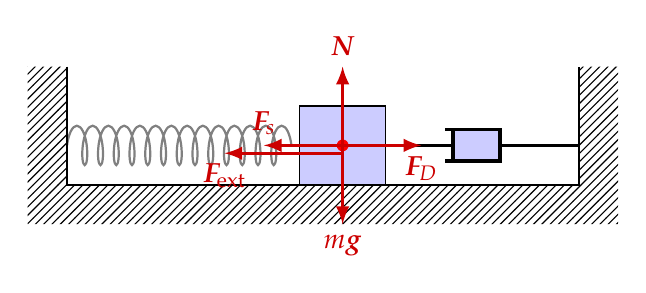
\begin{tikzpicture}
      \draw[fill=blue!20!white] (2.95,.5) rectangle(4.05,1.5);
      \draw[thick,draw=black!50,
        decoration={aspect=0.3,segment length=2mm, amplitude=2.5mm, coil},
        decorate] (0,1)--(2.95,1);
      \fill[pattern=north east lines](-.5,2)--(-.5,0)--(7,0)--(7,2)--(6.5,2)
      --(6.5,.5)--(0,.5)--(0,2)--cycle;
      \draw[thick] (0,2)--(0,.5)--(6.5,.5)--(6.5,2);
      \draw[fill=blue!20!white] (4.9,.8) rectangle(5.5,1.2);
      \begin{scope}[very thick]
        \draw(4.05,1)--(4.9,1);
        \draw(4.9,.8)--(4.9,1.2);
        \draw(4.8,1.2)--(5.5,1.2)--(5.5,.8)--(4.8,.8);
        \draw(5.5,1)--(6.5,1);
      \end{scope}
      \fill[red] (3.5,1)circle(.075);
      \begin{scope}[very thick,->,red!80!black]
        \draw (3.5,1)--(3.5,0) node[below]{$m\bm{g}$};
        \draw (3.5,1)--(3.5,2) node[above]{$\bm{N}$};
        \draw (3.5,1)--(2.5,1) node[above]{$\bm{F}_s$};
        \draw (3.5,.9)--(2,.9) node[below]{$\bm{F}_\text{ext}$};
        \draw (3.5,1)--(4.5,1) node[below]{$\bm{F}_D$};
      \end{scope}
    \end{tikzpicture}
  \end{center}
  Assume that the system is subjected to an external force that is sinusoidal
  with time, with a driving frequency $\omega$:

  \eq{-.2in}{
    F_\text{ext}=F_0\cos(\omega t)
  }  
\end{frame}



\begin{frame}{Forced Harmonic Motion}
  Accounting for all the forces in the $x$ direction, and applying the second
  law of motion:
  
  \eq{-.2in}{
    -kx-bv+F_0\cos(\omega t)=ma
  }

  This is a difficult problem (even for calculus students), but its solution is
  well known. It has:
  \begin{itemize}
  \item A \textbf{transient solution} identical to the damped oscillator
    \begin{itemize}
    \item Obtained by setting the external force term to zero
    \item Depends on the initial condition
    \item Solution becomes negligible over time because of exponential decay
    \end{itemize}
  \item A \textbf{steady-state solution} which does not depend on the initial
    condition
  \end{itemize}
\end{frame}



\begin{frame}{Forced Harmonic Motion}
  Solving for the steady-state solution is a difficult calculus exercise, but
  the solution is a harmonic motion at the driving frequency $\omega$ of the
  external force:

  \eq{-.2in}{
    \boxed{x(t)=A\cos(\omega t-\phi)}
  }
  
  The equation is in the same form as the SHM case, but the amplitude $A$ and
  phase shift $\phi$ are now given by:

  \eq{-.3in}{
    A=\frac{F_0}{\sqrt{m^2(\omega_0^2-\omega^2)^2+b^2\omega^2}}
    \quad\;\;
    \phi=\tan^{-1}\left[\frac{b\omega}{m(\omega_0^2-\omega^2)}\right]
  }
\end{frame}



\begin{frame}{Resonance}
  \textbf{Resonance} is caused by in-phase excitation at natural frequency.
  This means that:
  \begin{itemize}
  \item The frequency of the driving force is same as the natural frequency of
    the oscillator

    \eq{-.2in}{
      \omega=\omega_0=\sqrt{\frac{k}m}
    }
  \item The driving force follows the motion of the oscillator.
  \end{itemize}
\end{frame}



\begin{frame}{Resonance}
  Looking at the expression for amplitude of the oscillation:
  
  \eq{-.2in}{
    A=\frac{F_0}{\sqrt{m^2(\omega_0^2-\omega^2)^2+b^2\omega^2}}
  }
  
  Amplitude is at maximum when the frequency of the driving force $\omega$ is
  equal to the natural frequency $\omega_0$, with a maximum value of:
  
  \eq{-.2in}{
    A_\text{max}=\frac{F_0}{b\omega}
  }
\end{frame}



\begin{frame}{Resonance}
  \begin{columns}
    \column{.4\textwidth}
    \pic1{resonance-fig2}
    
    \column{.6\textwidth}
    Plotting amplitude $A$ as a function of driving frequency $\omega$ shows
    that:
    \begin{itemize}
    \item Resonance response is highest when $\omega=\omega_0$, which we know
      already
    \item The smaller the damping constant $b$, the higher and narrower the
      peak is
    \end{itemize}
  \end{columns}
\end{frame}



\begin{frame}{Resonance}

  \eq{-.01in}{
    \boxed{\tan\phi=\frac{b\omega}{m(\omega_0^2-\omega^2)}}
  }

  When $\omega=\omega_0$ is substituted into the phase shift expression, the
  right-hand side becomes undefined. From this, we obtain a phase shift of
  $\phi=\pi/2$. Using the expression for $v(t)$, and substituting $\phi=\pi/2$:
  
  \eq{-.2in}{
    v(t)=-A\omega\sin(\omega t-\frac{\pi}2)=A\omega\cos(\omega t)
  }
\end{frame}


\begin{frame}{Resonance}
  At resonance, the object is always moving in the same direction as the
  driving force:

  \vspace{-.4in}{\Large
    \begin{align*}
      v(t)&=A\omega\cos(\omega t)\\
      F_\text{ext}(t)&=F_0\cos(\omega t)
    \end{align*}
  }
\end{frame}

\end{document}
